\documentclass[11pt]{article}
% \def\hidesolutions{}
%%%%%%%%%%% SET MARGINS
\setlength{\textheight}{20cm}
\setlength{\topmargin}{-0.5cm}
\setlength{\oddsidemargin}{+0cm}
\setlength{\textwidth}{16.3cm}
%\setlength{\parskip}{6pt}
\setlength{\parindent}{0pt}

%%%%%%%%%%% PACKAGES
\usepackage{amsmath}
\usepackage{amssymb}
\usepackage{amsfonts}
%\usepackage{a4wide}
\usepackage{graphicx}
\usepackage{color}
\usepackage[normalem]{ulem}
\usepackage{enumitem}
\usepackage{capt-of}
\usepackage{float}
\usepackage{amsmath}
\usepackage{listings}
\definecolor{mygreen}{RGB}{28,172,0} % color values Red, Green, Blue
\definecolor{mylilas}{RGB}{170,55,241}
\usepackage{empheq}
\usepackage[ruled]{algorithm2e}
\usepackage{mathrsfs}
\usepackage{datetime}
\usepackage{subcaption}

% TODO: combine the two package lists and reduce redundancies 
\usepackage{mathtools}
\usepackage{nicefrac}
\usepackage{hyperref}
\usepackage{url}
\usepackage{amsmath,amssymb,amsfonts}
\usepackage{a4wide}
\usepackage{graphicx}
\usepackage{color}
\usepackage[normalem]{ulem}
\usepackage{capt-of}
\usepackage{float}
\usepackage[ruled]{algorithm2e}
\usepackage{amsmath,amssymb,amsfonts}
\usepackage{a4wide}
\usepackage{graphicx}
\usepackage{color}
\usepackage[normalem]{ulem}
\usepackage{capt-of}
\usepackage{float}
\usepackage[ruled]{algorithm2e}
\usepackage{mathrsfs}







\newcommand{\Lc}[2]{{\color{blue} \sout{#1} } \textcolor{red}{#2}}
\newcommand{\La}[1]{\textcolor{red}{#1}}
\newcommand{\lh}{\mathscr{L}_h}
\newcommand{\cl}{\mathscr{L}}
\newcommand{\cf}{\mathscr{F}}
\newcommand{\dx}{dx}
\newcommand{\ltn}{\mathscr{l}^2}
\newcommand{\bbR}{\mathbb{R}}
\newcommand{\Rset}{\mathbb{R}}
\newcommand{\Nset}{\mathbb{N}}
\newcommand{\scL}{\mathcal{L}}
\newcommand{\xx}{\mathbf{x}}
\newcommand{\norm}[1]{\|{#1}\|}
\newcommand{\yy}{\mathbf{y}}
\newcommand{\at}[1]{\big|_{#1}}
\renewcommand{\div}{\mathrm{div}}
\newcommand{\divergence}{\mathrm{div}}
\newcommand{\cp}[1]{\textcolor{blue}{#1}}

\newcommand{\FF}{\texttt{FreeFem++ }}
\newcommand{\FFns}{\texttt{FreeFem++}}
\newcommand{\FFfull}{\texttt{FreeFem++-x11}}
\newcommand{\cmd}[1]{ \medskip \noindent \texttt{#1} \medskip}
\newcommand{\incmd}[1]{\texttt{#1}}
\newcommand{\shrinkitems}{\addtolength{\itemsep}{-0.5\baselineskip}}
\newcommand{\mtt}[1]{\mathtt{#1}}
\newcommand{\ML}{\texttt{Matlab }}

\newcommand{\bb}{\mathbf{b}}
\newcommand{\nn}{\mathbf{n}}
\newcommand{\vecA}{\vec{A}}
\newcommand{\vecB}{\vec{B}}


\newcommand{\mesh}{\mathcal{T}_h}
\newcommand{\refel}{\widehat{K}}
\newcommand{\ver}{\mathbf{a}}
\newcommand{\refver}{\widehat{\mathbf{a}}}
\newcommand{\grad}{\nabla}
\newcommand{\refgrad}{\widehat{\nabla}}
\newcommand{\refu}{\widehat{u}}
\newcommand{\refbasis}{\widehat{\varphi}}
\newcommand{\refxx}{\widehat{\xx}}
\newcommand{\refx}{\widehat{x}}
\newcommand{\refy}{\widehat{y}}
\newcommand{\refrho}{\widehat{\rho}}
\newcommand{\refh}{\widehat{h}}






% For typesetting Python code
\newcommand{\matlab}{{\sc Matlab}\xspace}
\usepackage{listings}
\lstloadlanguages{Python}
\lstloadlanguages{csh}%
\definecolor{MyDarkGreen}{rgb}{0.0,0.4,0.0}
\definecolor{purple}{rgb}{0.58,0,0.82}
\lstset{language=Python,                    % Use Python
	%frame=single,                          % Single frame around code
	basicstyle=\ttfamily\footnotesize\color{black},
	keywordstyle=[1]\color{blue}\bf,        % Python functions bold and blue
	keywordstyle=[2]\color{purple},         % Python function arguments purple
	keywordstyle=[3]\color{red}\underbar,   % User functions underlined and blue
	commentstyle=\usefont{T1}{pcr}{m}{sl}\color{MyDarkGreen}\small,
	stringstyle=\color{purple},
	showstringspaces=false,                 % Don't put marks in string spaces
	tabsize=3,                              % 5 spaces per tab
	morekeywords={xlim,ylim,var,alpha,factorial,poissrnd,normpdf,normcdf},
	morecomment=[l][\color{blue}]{...},
	breaklines=true,
	breakatwhitespace=true,
	emptylines=1,
	mathescape=true,
	xleftmargin=0ex,
	emphstyle=\bfseries\color{red}
}





%%%%%%%%%%% MACROS NAMES
\newcommand{\lecturername}{Martin Licht}
% \newcommand{\assistantnamea}{Jochen Hinz}
% \newcommand{\assistantnameb}{Ivan Bioli}
\newcommand{\semestername}{Winter Semester 2023}
\newcommand{\lecturename}{Analysis III - 202(c)}
\DeclarePairedDelimiter\floor{\lfloor}{\rfloor}

%%%%%%%%%%% HEADER
\newdateformat{yeardate}{\THEYEAR}
\newcommand{\exsheet}[3] % input is the number of the session and the day TODO What's that
{\clearpage

	\begin{center}
		{\Large \textbf{\lecturename}}\\[2ex]
		\semestername
	\end{center}

	% \vspace{2ex}
	% \lecturername

	\vspace{2ex}
	{\Large Session #1: #3\,#2, \yeardate\today}
	%\hfill
	%{\Large EPF Lausanne}

	\hrulefill
}





\usepackage{comment}

\newtheorem{exercise}{Exercise}
\newtheorem{solutionenv}{Solution}

\newboolean{hide_solution}
\ifx\hidesolutions\undefined
\newenvironment{solution}{\begin{solutionenv}}{\end{solutionenv}}
\setboolean{hide_solution}{false}
\else
\excludecomment{solution}
\setboolean{hide_solution}{true}
\fi

\newcommand{\ifnotsolution}[1]{\ifthenelse{\boolean{hide_solution}}{#1}{}}
\newcommand{\ifsolution}[1]{\ifthenelse{\boolean{hide_solution}}{}{#1}}








\allowdisplaybreaks

\begin{document}
\exsheet{3}{26}{September} % parameters are the number of the session and the day


% \begin{exercise}
%     We have focused on scalar and vector fields that are defined on the entire space. 
%     But sometimes we are also interested in fields with singularities. 
%     Compute the gradient and the Laplacian of the function 
%     \[
%         f : \bbR^3 \setminus \{0\} \rightarrow \bbR, \quad (x_1,x_2,x_3) \mapsto \frac{1}{\sqrt{x_1^2+x_2^2+x_3^1}}
%     \]
%     where the scalar field is twice differentiable. 
%     Sketch the gradient field.
% \end{exercise}
% \begin{solution}   
%     $$
%         \grad f(x_1,x_2,x_3)
%         =
%         -\frac{1}{(x_1^2+x_2^2+x_3)^{\frac{3}{2}}} \begin{pmatrix}x_1\\ x_2\\\frac{1}{2}\end{pmatrix}
%     $$ 
%     \begin{align*}
%         \Delta f(x_1,x_2,x_3) 
%         &=
%         \nabla \cdot \nabla f(x_1,x_2,x_3) 
%         \\
%         &= \frac{\partial}{\partial x_1}\left(-\frac{x_1}{(x_1^2+x_2^2+x_3)^{\frac{3}{2}}} \right)
%         + \frac{\partial}{\partial x_2}\left(-\frac{x_2}{(x_1^2+x_2^2+x_3)^{\frac{3}{2}}}\right)
%         + \frac{\partial}{\partial x_3}\left(-\frac{1}{2(x_1^2+x_2^2+x_3)^{\frac{3}{2}}} \right)
%         \\
%         &= 
%         - \frac{2}{(x_1^2+x_2^2+x_3)^{\frac{3}{2}}}
%         + \frac{6x_1^2 + 6x_2^2}{(x_1^2+x_2^2+x_3)^{\frac{5}{2}}}
%         + \frac{3}{4(x_1^2+x_2^2+x_3)^{\frac{5}{2}}}
%         \\
%         &=
%         \frac{4x_1^2 + 4x_2^2 -8x_3 +3}{4(x_1^2+x_2^2+x_3)^{\frac{5}{2}}}
%     \end{align*}
% \end{solution}

\begin{exercise}
    Consider the scalar field $f(x_1,x_2) = x_1 x_2$. 
    \begin{itemize}
     \item Describe its level sets for the values $-2, -1, 0, 1, 2$.
     \item Draw the gradient at a few points, such as 
     \begin{align}
        \left( 1,0 \right), \left( 0,1 \right), \left( 1,1 \right), \left( -1,-1 \right), \left( \sqrt{2},\sqrt{2} \right), \left( \sqrt{2},-\sqrt{2} \right)
     \end{align}
     \item 
     Recall the hyperbolic sine and hyperbolic cosine functions $\sinh(t)$ and $\cosh(t)$. 
     Sketch the curve 
     \begin{align}
        \gamma : (-\infty,\infty) \rightarrow \bbR^{2}, \quad t \mapsto \left( \; \cosh(t), \; \sinh(t) \; \right)
     \end{align}
     and compute its tangent vector $\dot \gamma$.
    \end{itemize}
\end{exercise}
\begin{solution}
    The figure in total has got the following shape:
    \begin{figure}[h]
    \centering
    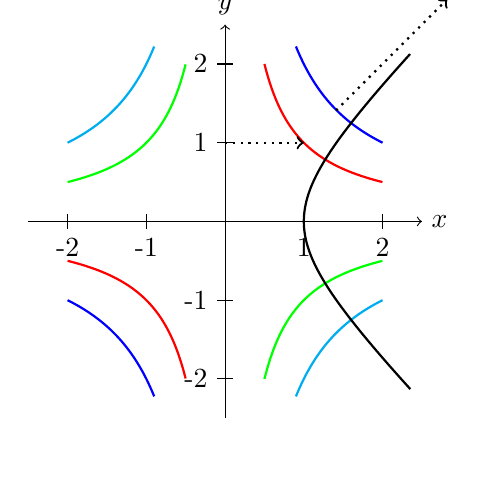
\begin{tikzpicture}[scale=1.0]
        \draw[->] (-2.5,0) -- (2.5,0) node[right] {$x$};
        \draw[->] (0,-2.5) -- (0,2.5) node[above] {$y$};
        \foreach \x in {-2,-1,1,2}
        \draw (\x,0.1) -- (\x,-0.1) node[below] {\x};
        \foreach \y in {-2,-1,1,2}
        \draw (0.1,\y) -- (-0.1,\y) node[left] {\y};

        \draw[domain=  0.5:2, samples=100, smooth, thick,red] plot (\x,1/\x) node[right] {};
        \draw[domain=-2:-0.5, samples=100, smooth, thick,red] plot (\x,1/\x) node[right] {};
        \draw[domain=  0.9:2, samples=100, smooth, thick,blue] plot (\x,2/\x) node[right] {};
        \draw[domain=-2:-0.9, samples=100, smooth, thick,blue] plot (\x,2/\x) node[right] {};
        \draw[domain=  0.5:2, samples=100, smooth, thick,green] plot (\x,-1/\x) node[right] {};
        \draw[domain=-2:-0.5, samples=100, smooth, thick,green] plot (\x,-1/\x) node[right] {};
        \draw[domain=  0.9:2, samples=100, smooth, thick,cyan] plot (\x,-2/\x) node[right] {};
        \draw[domain=-2:-0.9, samples=100, smooth, thick,cyan] plot (\x,-2/\x) node[right] {};
        
        \draw[domain=-1.5:1.5, samples=100, smooth, thick] plot ({cosh(\x)},{sinh(\x)}) node[right] {};
        
        \draw[thick,dotted,->] (0,1) -- (1,1);
        \draw[thick,dotted,->] (1.41,1.41) -- (2.82,2.82);

        \end{tikzpicture}     
    \end{figure}
    \begin{enumerate}
     \item 
     \item 
     \item 
    \end{enumerate}
\end{solution}



\begin{exercise}
    Consider the curves 
    \[
        \gamma : [-1,1] \rightarrow \bbR^2, \quad t \mapsto ( t^3, t^2 )
    \]
    \[
        \delta : [-1,1] \rightarrow \bbR^2, \quad t \mapsto ( \cos(t), \sin(2t) )
    \]
    Draw them. Are they simple, closed, differentiable, or regular? What are their tangents?
    
    Show that $\gamma$ is the graph of a function in the first coordinate.
\end{exercise}
\begin{solution}    
    For the first curve the tangent is given by $\dot{\gamma}(t) = ( 3t^2, 2t )$.
    Moreover the curve is simple (it does not intersect itself), differentiable and regular (since $\dot{\gamma} \neq \vec{0}$).
    \\

    For the second curve we have the tangent is given by $\dot{\delta}(t) = (-sin(t),2cos(2t))$.
    Moreover the curve is simple (it does not intersect itself), differentiable and regular (since $\dot{\delta} \neq \vec{0}$).
\end{solution}

\begin{exercise}
    Compute the line integral of
    \[
        f : \bbR^2 \to \bbR, \quad (x_1,x_2) \mapsto 1 + x_1^2 + x_2^2
    \]
    along the two curves $\gamma$ and $\delta$, given by 
    \[
        \gamma : [0,\pi] \rightarrow \bbR^2, \quad t \mapsto ( -\cos(t), \sin(t) )
    \]
    \[
        \delta : [-1,1] \rightarrow \bbR^2, \quad t \mapsto (t,0)
    \]
    Compare the results. What are the endpoints of the two curves? 
\end{exercise}
\begin{solution}     
    \begin{align*}
        \int_{\Gamma} f(x_1,x_2) d\ell 
        &= \int_{0}^{\pi} ( 1 + \cos(t)^2 + \sin(t)^2 ) |\dot{\gamma}(t)|dt
        \\&= \int_{0}^{\pi} ( 1 + \cos(t)^2 + \sin(t)^2 ) \sqrt[]{\cos(t)^2 + \sin(t)^2} dt
        \\&= \int_{0}^{\pi} ( 1 + 1 ) \sqrt[]{1} dt
        \\&= \int_{0}^{\pi} 2 dt
        \\&= 2\pi.
    \end{align*}
    The endpoints of the first curve are: $\gamma(0) = (-1,0)$ and $\gamma(\pi) = (1,0)$.

    Let us now compute the second integral. We see 
    \begin{align*}
        \int_{\Gamma} f(x_1,x_2) d\ell 
        &= \int_{-1}^{1} (f\circ \delta)(t)|\dot{\delta}(t)|dt
        \\&= \int_{-1}^1 (1+t^2)\left|\begin{pmatrix} 1\\0 \end{pmatrix}\right| dt
        \\&= \int_{-1}^1 (1+t^2) dt
        \\&= 2 \int_{0}^1 (1+t^2) dt
        \\&= 2\left[t+\frac{t^3}{3} \right]_{0}^{1}
        \\&= \frac 8 3.
    \end{align*}
    Note that from the third to fourth line, we have used that the integrand was even. 
    The endpoints of the second curve are: $\delta(-1) = (-1,0)$ and $\delta(1) = (1,0)$.

    The exercise also shows that integrating a function $f$ along different curves may give different results, 
    even if the curves share the same starting and endpoints. 
\end{solution}

\begin{exercise}
    Compute the line integral of $f : \bbR^2 \rightarrow \bbR$ 
    along the circle $C$ with radius $3$ centered at the origin, where 
    \[
        f : \bbR^2 \to \bbR, \quad (x_1,x_2) \mapsto 3 x_2^2 + x_2^3
    \]
    Hint: you must first find a parameterization of $C$. 
\end{exercise}
\begin{solution} 
	We may choose the following parameterization for the circle $C$:
    $$
        \gamma : [-\pi,\pi] \rightarrow \bbR^2, \quad t \mapsto ( 3\cos(t), 3\sin(t) )
    $$
    \begin{align*}
        \int_{\Gamma} f(x_1,x_2) d\ell &= \int_{-\pi}^{\pi} (f\circ \gamma)(t)|\dot{\gamma}(t)|dt
        \\&=
        \int_{-\pi}^{\pi} \left[3(3\sin(t))^2+(3\sin(t))^3)\right]\left|\begin{pmatrix}3\cos(t)\\3\sin(t)\end{pmatrix}\right| dt
        \\&=
        \int_{-\pi}^{\pi} 3\left[27\sin^2(t)+27\sin^3(t))\right]dt
        \\&=
        81\int_{-\pi}^{\pi} \sin^2(t)dt+ 81\int_{-\pi}^{\pi}\sin^3(t))dt\\
    \end{align*}
    The second integral is $0$ since the integrand is uneven. For the first integral we use the cosine half-angle formula ($1 - 2\sin^2(\alpha) = \cos(2\alpha)$).
    \begin{align*}
        &= 81\int_{-\pi}^{\pi} \frac{1}{2} - \frac{1}{2}\cos(2t)dt
        \\&= 81 \left[ \frac{1}{2} t - \frac{1}{4}\sin(2t) \right]_{-\pi}^{\pi} = 81\pi
    \end{align*}
    % Pick a parameterization, use that one integrand is odd and therefore vanishes, and use the cosine half-angle formula for the other term.
\end{solution}

\begin{exercise}
    You are excavating a tunnel deep beneath surface through rock from a point $A=(-1,0)$ to a point $B=(1,1)$ along a curve $\Gamma$.
    Geological observations show that the rock mass density of the region can be modeled by 
    \[
        f(x_1,x_2) = \exp(x_1+x_2).
    \]
    The costs and abbrasion of the tools are therefore proportional to the curve integral
    \[
        \int_\Gamma f \; dl
    \]
    Compute the integral along the straight line 
    \[
        \gamma : [0,1] \rightarrow \bbR^2, \quad t \mapsto (-1+2t, t)
    \]
\end{exercise}
\begin{solution}
    We set up the first curve integral and compute:
    \begin{align*}
        \int_\Gamma f \cdot dl
        &=
        \int_0^1 \exp(-1+2t+t) \|(2,1)\| dt
        \\&=
        \int_0^1 \exp(-1+2t+t) \sqrt{5} dt
        \\&=
        \sqrt{5} \int_0^1 \exp(3t-1) dt
        \\&=
        \frac{\sqrt{5}}{3} 
        \int_0^1 3 \exp(3t-1) dt
        \\&=
        \frac{\sqrt{5}}{3} 
        \Big[ \exp(3t-1) \Big]_0^1
        =
        \frac{\sqrt{5}}{3} 
        \left( \exp(2) - \exp(-1) \right)
        =
        \frac{\sqrt{5}}{3} 
        \left( e^2 - \frac{1}{e} \right)
        .
    \end{align*}
\end{solution}


\begin{exercise}
    A matrix $A \in \bbR^{n \times n}$ is called symmetric if $A = A^{t}$ and antisymmetric if $A = - A^{t}$. 
    \begin{enumerate}
     \item Show that a matrix that is both symmetric and antisymmetric must be zero.
     \item Show that every matrix $B \in \bbR^{n \times n}$ can be written as a sum $A = A_1 + A_2$ where $A_1 \in \bbR^{n \times n}$ is symmetric and $A_2 \in \bbR^{n \times n}$ is antisymmetric. 
     \item Let $f : \bbR^{n} \rightarrow \bbR$ be a scalar field with continuous partial derivatives up to second order. 
     Show that its Hessian is a symmetric matrix.
     \item The \emph{trace} of a matrix is the sum of its diagonal elements. Find a scalar field in $\bbR^{2}$ whose Hessian is not zero but has zero trace.
     \item Let $F : \bbR^{2} \rightarrow \bbR^{2}$ be a differentiable vector field. What is the antisymmetric part of its Jacobian?
     \item Let $G : \bbR^{3} \rightarrow \bbR^{3}$ be a differentiable vector field. What is the antisymmetric part of its Jacobian?
     \item What do you notice in the answers to the last two questions?
    \end{enumerate}
\end{exercise}
\begin{solution}
    \begin{enumerate}
     \item 
     \item 
     \item 
     \item We can use $f(x_1,x_2) = x_1 x_2$.
     \item 
     \item 
     \item We notice that the entries in the antisymmetric parts of the Jacobians contain already all the information for the curl of the respective vector fields (in 2D and 3D). More generally, we can define the curl of a vector field $F : \bbR^{n} \rightarrow \bbR^{n}$ as the antisymmetric part of the Jacobian.
    \end{enumerate}
\end{solution}




%\begin{exercise}
%    Compute the line integral of $f : \bbR^2 \rightarrow \bbR$ 
%    along the circle $C$ with radius $3$ centered at the origin, where 
%    \[
%        f : \bbR^2 \to \bbR, \quad (x_1,x_2) \mapsto 3 x_2^2 + x_2^3
%    \]
%    Hint: you must first find a parameterization of $C$. 
%\end{exercise}
%\begin{solution}     
    % Pick a parameterization, use that one integrand is odd and therefore vanishes, and use the cosine half-angle formula for the other term.
%\end{solution}


\end{document}
